% X = [0,1] with points 1/n; the quotient X/A is a wedge of shrinking circles.
% Source: book/tex/homology/excision.tex (§ Motivating relative homology).
\documentclass[border=2mm]{standalone}
\usepackage{tikz}
\usetikzlibrary{arrows.meta}
\begin{document}
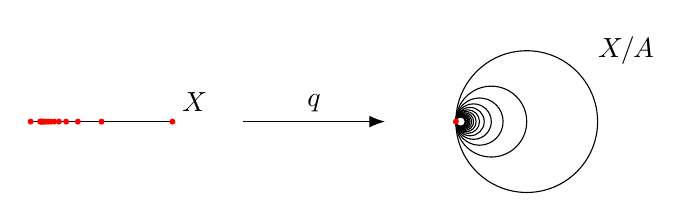
\begin{tikzpicture}[>={Latex[length=2mm]}, scale=1.8]
  \draw (0,0)--(1,0) node[above right] {$X$};
  \fill[red] (0,0) circle (0.6pt);
  \foreach \n in {1,...,15} {\fill[red] ({1/\n},0) circle (0.6pt);}
  \draw[->] (1.5,0)--(2.5,0) node[midway,above] {$q$};
  \foreach \n in {1,...,15} {\draw ({3+1/(2*\n)},0) circle ({1/(2*\n)});}
  \fill[red] (3,0) circle (0.6pt);
  \node at (4.2,0.5) {$X/A$};
\end{tikzpicture}
\end{document}
